\chapter{Pyramid Match Score for Detection}
\label{chp5}

\section{Introduction}

Bag-of-features~\cite{bgf} schema can be considered as the watershed between traditional and modern detection methods. Instead of considering each target object as a collection of raw optical elements, i.e., pixels, the schema tries to consider each object as a set of semantic elements or so-called object parts which are usually some strong local image features. Then one visual object is said to be a target object if it possesses some certain local features of certain numbers, while does not contain other certain local features of certain numbers. While this is quite straightforward, the very precious information encoded in local features' relative positions is left over. Following some pioneering ideas~\cite{spmk,ac30}, this chapter proposes a detection method which combines spatial and visual information of local image features in a  way pursuing both efficiency and effectiveness.

The results of Chapter \ref{chp4} is promising on the two experimental datasets, however, the efficiency is not good due to the employment of Hough transform framework.
 Besides, inferring object status in a bottom-up manner fails to capture global information of each target object from the very beginning. And this is also why recently the detection results of Hough transform based methods need refinement by discriminative methods in order to be competitive. Still the way how to use spatial information of local features is very illuminate. 
 
 Just as said in~\cite{ac27}, Hough transform based methods and sliding-window methods are the two sides of the same coin. The method proposed in this chapter calculates confidence of a target object class for each sub-window in an image. Instead of considering each object as a collection of visual patterns (appearance of local features), the method considers each object as a set of visual-spatial patterns. One object is considered as a set of points. Each point is a digital vector, with the last two dimensions the relative $x-$ and $y-$ coordinates to object center, and SIFT after principle component analysis as the remaining dimensions. The training procedure is about collecting all such visual-spatial points into a point set, which acts as a super template. During detection, each sub-image is considered as a point set, and it is matched against the super template. The confidence is then the match score.
 
 The key to this method is how to define a matric or match score for two point sets. Here pyramid matching procedure is employed, not only for efficiency, but also for combining visual and spatial information from local features in an effective manner. The visual-spatial space is divided from fine to coarse. Under a certain dividing parameter, points from the two matching point sets are considered as match if they fall into the same grid, and they are excluded from the respective point sets. The procedure continues till one point set is empty. Then the numbers of matched pairs under each dividing method is counted, and a weighted sum of all these numbers are considered as the match score for two point set, which will be referred to as Pyramid Match Score, or PMS for short. The weights under all dividing methods are learned during training, and also how to divide the visual-spatial space is of great importance.
 
Obviously, each object is considered as a whole during detection in this method.

The proposed method also has several appealing properties, which include but not limited to:
\begin{itemize}
\item {Feasibility of sequential/batch training, which will lead to easy deployment in distributed system.}
\item {Space complexity of the model is $O(1)$. Since the capacity of the point set acting as the super template is finite, and the size of the model is limited by the capacity.}
\item {Detection time complexity not related to the size of training examples.}
\end{itemize}

This chapter is organized as follows. Section \ref{rw5} reviews most related work. Section \ref{dt5} propose the training and detecting procedure. Section \ref{exp5} gives experimental results. Section \ref{conc5} concludes this chapter.

\section{Related Work}
\label{rw5}


Detection methods still mainly follow the sliding-window schema or share similar structures with Hough transforms. While the focus of the later is to infer about object status by use each online feature as query against a well-trained codebook. These methods fail to consider target objects as a whole at the beginning. The problem of sliding-window is that it often ignores positional information when also following bag of features~\cite{bgf}. In the method of~\cite{spmk}, positional information is considered in the kernel function. Here a kernel function is usually used in classifiers, which are usually support vector machines, as introduced in~\cite{kmts}. The assumption behind~\cite{spmk} is that two images are considered as similar if they possess similar object parts at similar relative positions. Despite of the good theory, its being embedded in support vector machines as kernel function limits the efficiency of this method.


The Bag-of-features~\cite{bgf} schema successfully improves detection performance, while still there are information which are left behind in images. The positional information is not fully made use of, even the method of~\cite{kmts}. While~\cite{uspl} provides a method to model the relationship between object parts, there are two many parameters to estimate in their model, which requires large amount of training data for acceptable performance.

In the method proposed in~\cite{ac222}, each object is modeled as a graph, when matching each object with another, constrains are made not only between the two objects, but also between different features of the same object. The relationship between elements of the same object is important. However, the inefficiency of this method prevents it from directly being used for object detection, while its performance on matching the same object under different views is promising.

The method in~\cite{lbt1} instead of building some parametric or non-parametric model, directly maps the labels of similar images in the training images to the current image. In this manner, the descriptive ability of model can be left alone, which in return makes the method robust. However, this kind of methods heavily rely on the manually marked labels in the training dataset, while such labels are very expensive in human power and computation.

The method in~\cite{ac3} considers both appearance model of object parts, and the relative distance changes between object parts. While giving promising results, there are too many parameters in the model, and training is troublesome when limited training images are available.

The successes of HOG~\cite{ij4} on pedestrians are also because of its ability to encode relative spatial and visual information from each divided cells. Still the flexibility is not enough, and this leads to deformable part model~\cite{ac30,ac31,dpm1,dpm2}, which will be referred as DPM for short, is currently employed by most state-of-the-art methods which consider  appearance information of object parts together with the relative positional information between object parts. A root template is used to detect object as a whole, and HOG feature is usually used. When an object is detected, all possible object parts are detected accordingly. Finally, the confidence is given by the confidence of the root object, the sum of confidence of the object parts, and the cost to deploy the object parts within the root object. Latent SVM is employed in the methods for optimization while using representation of complex information. Some methods motivated by DPM try to improve DPM by providing better solution searching strategies~\cite{dpm3}.  Two recent methods~\cite{spm,spltm} try to find sparse basis of object parts to reduce the number of parameters need estimating. For efficiency, the method in~\cite{408} replace the dot operator of DPM with start-of-the-art hashing method~\cite{lsh}. There also exists hierarchical extend of DPM~\cite{hdpm}, and multi-view extend of DPM~\cite{mvdpm}.

Advantages of DPM include that it only need to encode the object parts in positive training examples, and that the some of its invariants can give promising results in real time. Still DPM heavily rely of the latent SVM, which is trained in an  expectation�Cmaximization manner stops it from adopting new training examples. While nowadays, training examples often come sequentially. A very flexible model, which will evolve with training examples is preferred. These evolvements include object part number evolving, evolving of the appearance models of object parts, and evolving of the relative positions of object parts.



The pyramid match score method is most related to methods using~\cite{pmk} or~\cite{kmts} as kernel functions, methods employ Hough transforms, and also the methods proposing efficient solution space searching techniques~\cite{bab}. The method is also related to efforts trying to encode images~\cite{spen}.





\subsection{Pyramid Matching}



The Pyramid Matching method is designed to find the best one-one match, as shown in Figure \ref{fig:p2}, between two point sets in a heuristic manner.

Given two point sets, ${S_1} = \{ {u_1},{u_2},...,{u_m}\}, u_i \in {R^d}
$
 and ${S_2} = \{ {v_1},{v_2},...,{v_n}\}, v_i \in {R^d}$
, there exists a best one-one matching ${\pi}^*$ that minimizes the sum of $L1$
-distances between matched pairs,

\[
{\pi ^*} = \arg \mathop {\min }\limits_\pi  \sum\limits_{{u_i} \in {S_1}} {||{u_i} - {v_{\pi (i)}}|{|_1}} \ .
\]
Here $m  \le n$, and $\pi$ maps each feature $u_i$ in $S_1$ to a unique feature ${{v_{\pi (i)}}}
$ in $S_2$. There is a 2D example in Figure \ref{fig:pms1}

The best matching exists, and can be found by simple brute-force enumeration. In special cases, the Hungarian algorithm~\cite{ha} is also applicable.

\begin{figure}
\centering
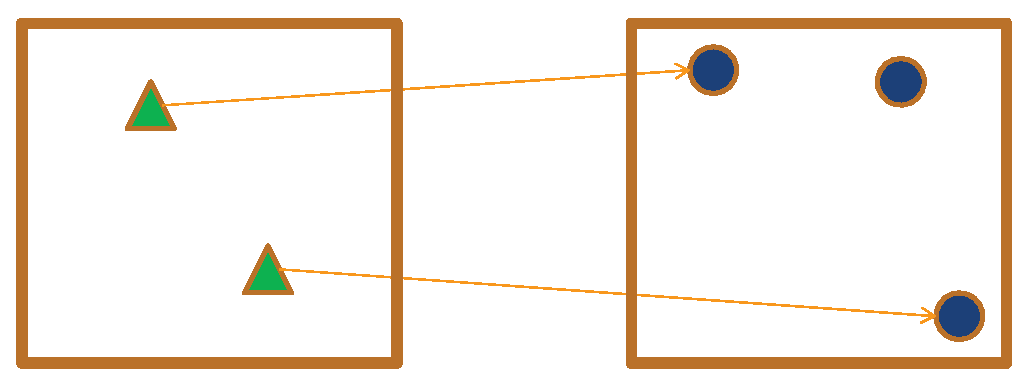
\includegraphics[width=1\textwidth]{pms1.eps}
\caption[Best one-one match.]{A best one-one match problem in 2D space. There are two points in the first point set, three in the second point set. The arrows show correspondence between the two point set.}
\label{fig:pms1}
\end{figure}

\begin{figure}
\centering
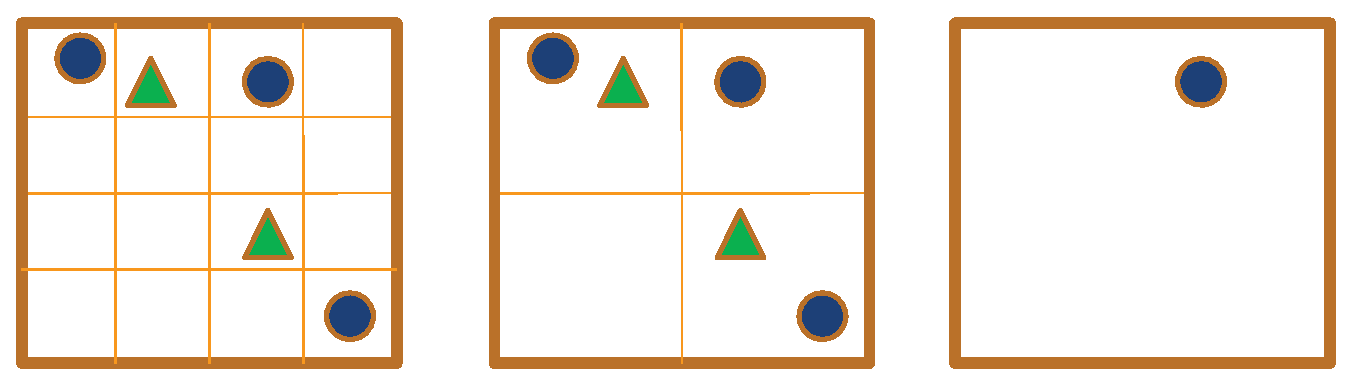
\includegraphics[width=1\textwidth]{pms2.eps}
\caption[Pyramid matching procedure.]{Pyramid matching procedure which takes the 2D one-one match problem in Figure \ref{fig:pms1} as an example. The pyramid matching method divides the 2D space from fine to coarse in the 2D space. Notice, the triangle points belong to point set one, and the circle points belong to point set two. In the left, each dimension is divided into 4, results in totally 16 grids, and no matched point pairs are found. In the middle, each dimension is divided into 2, results in totally 4 grids, and two pairs of points belonging to different point sets are found and excluded. In the right, since the matched points belonging to matched point pairs are excluded, then only one point from the second point set is left. So the number of pairs found under all dividing methods are, 0, 2, and 0. The pyramid match score is calculated as a weighted sum of these 0, 2, and 0. }
\label{fig:p2}
\end{figure}




Sub-optimal solution can be found by heuristic methods. A very intuitionistic method is to find matched pairs of nearest distance, exclude corresponding points from both point sets, and repeat until no matched pair can be found.

The Pyramid Matching method is straightforward. Divide the point space from fine to coarse, find pairs of points from different point sets in the same grid under the current dividing parameter, exclude the matched pairs, and continue this procedure until the smaller point set is empty. The Pyramid Matching method is very efficient, and its time complexity is bounded by $O(dmL)$~\cite{pmk}. Here $d$ is the number of dimensions in each point set, $m$ is size of the smaller point set, and $L$ is number of dividing methods. In the example of Figure \ref{fig:p2}, $L$ is 3.

In~\cite{pmk}, pyramid matching helps to define kernel functions for SVMs. The meaning of pyramid matching is that, it changes how the way to define similarity between two objects. Originally two objects are considered as similar if they both contain certain number of certain object parts, while the idea of one-one match will only favor the objects parts which have corresponding counterparts. 

Let $\gamma  = \{ {\bf{g}_1},{\bf{g}_2},...,{\bf{g}}_L\}$ be an ordered set, which contains all the dividing methods from fine to coarse. Let $N(S_1,S_2;{\bf{g}}_i)$ be the number of matched pairs of points under dividing method ${\bf{g}}_i$. Then the pyramid match score between $S_1$ and $S_2$ on $\gamma$ is defined by,

\begin{equation}
{\rm P}(S_1,S_2;\gamma)=\frac{{\omega}_1 \times N(S_1,S_2; {\bf{g}}_1) + \sum\limits^L_{i=2}{{\omega}_i\times( N(S_1,S_2;{\bf{g}}_i)-N(S_1,S_2;{\bf{g}}_{i-1}) ) }}{m}
.
\label{eq:pms1}
\end{equation}


Left behind is how to construct the dividing methods in $\gamma$ and how to define the corresponding weight ${\omega}_i$ for each ${\bf{g}}_i \in \gamma$. 
And these are also the two factors which lead to differences to~\cite{pmk}.


\subsection{Pyramid Match Score for Detection}

The Pyramid Match Score is a matric between two point sets. In~\cite{pmk}, image features are considered as points, while in the proposed method, each point encodes both appearance and location information of each local feature. 

Instead of following~\cite{pmk}, PMS does not server as kernel functions for SVMS. And, a procedure similar to Hough transform is employed. Each training image is also a point set, and the $+$ operator is well defined for two sets. From all the training images, we generate a point set as a super template, $S_{\bf{T}}$, following Algorithm \ref{alg:tm}. This is just a procedure to collect all point sets of training images into one point set.
Here each $S_{I_i}$ in $\{S_{I_i}\}$ is the point set generated from the corresponding training image $I_i$.

\begin{algorithm}[h]

    \caption{Template Generation}
    \label{alg:tm}
     



    \begin{algorithmic}[1]


       \STATE $S_{\bf{T}} \leftarrow \emptyset$
        
        \FOR{$S_{I_i} \in \{S_{I_i}\}$}
        
     \STATE  $S_{\bf{T}} \leftarrow S_{\bf{T}} + S_{I_i}$
       
        \ENDFOR

        
    \RETURN $S_{\bf{T}}$

    \end{algorithmic}

\end{algorithm}

Here, $S_{\bf{T}}$ plays a role similar to a codebook as in methods based on Hough transform. Each point is $d-$dimensional, here, the first $d-2$ dimensions are SIFT after PCA, while the last 2 dimension are relative $x-$ and $y-$ coordinates after considering scale and width-height ratio changes. 

For detection, a most popular pipeline is summarised, as in.


\begin{figure}
\centering
\includegraphics[width=1\textwidth]{pms3.eps}
\caption[Visual-spatial space dividing.]{Methods to divide the visual-spatial space.}
\label{fig:p3}
\end{figure}

\section{Detection}
\label{dt5}

Sliding-window schema is employed to check with the defined Pyramid Match Score on all sub-images of the test image for detection decisions.

\section{Experimental Results}
\label{exp5}


\begin{figure}
\centering

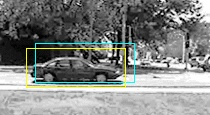
\includegraphics[scale=0.75]{test-0_good.jpg}
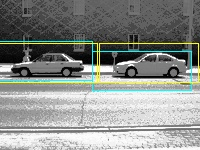
\includegraphics[scale=0.75]{test-10_good.jpg}
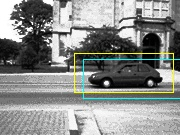
\includegraphics[scale=0.75]{test-14_good.jpg}
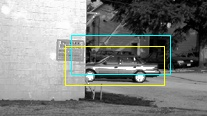
\includegraphics[scale=0.75]{test-16_good.jpg}
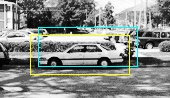
\includegraphics[scale=0.75]{test-20_good.jpg}
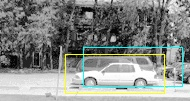
\includegraphics[scale=0.75]{test-21_good.jpg}
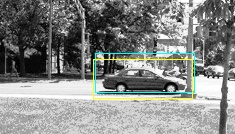
\includegraphics[scale=0.75]{test-22_good.jpg}
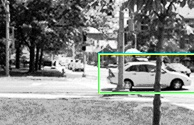
\includegraphics[scale=0.75]{test-24_good.jpg}
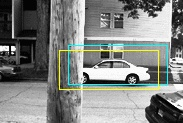
\includegraphics[scale=0.75]{test-29_good.jpg}
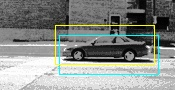
\includegraphics[scale=0.75]{test-2_good.jpg}
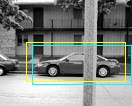
\includegraphics[scale=0.75]{test-31_good.jpg}
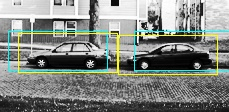
\includegraphics[scale=0.75]{test-3_good.jpg}
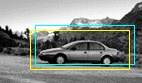
\includegraphics[scale=0.75]{test-5_good.jpg}


\caption[Detection Results on UIUC cars]{Detection results on UIUC cars~\cite{cds}. Yellow color marks ground truths, while blue marks detections.}
\label{fig:c5r}
\end{figure}

In Figure \ref{fig:c5r}, are some good results on UIUC cars. And new experiments will be added.
\begin{figure}
\centering

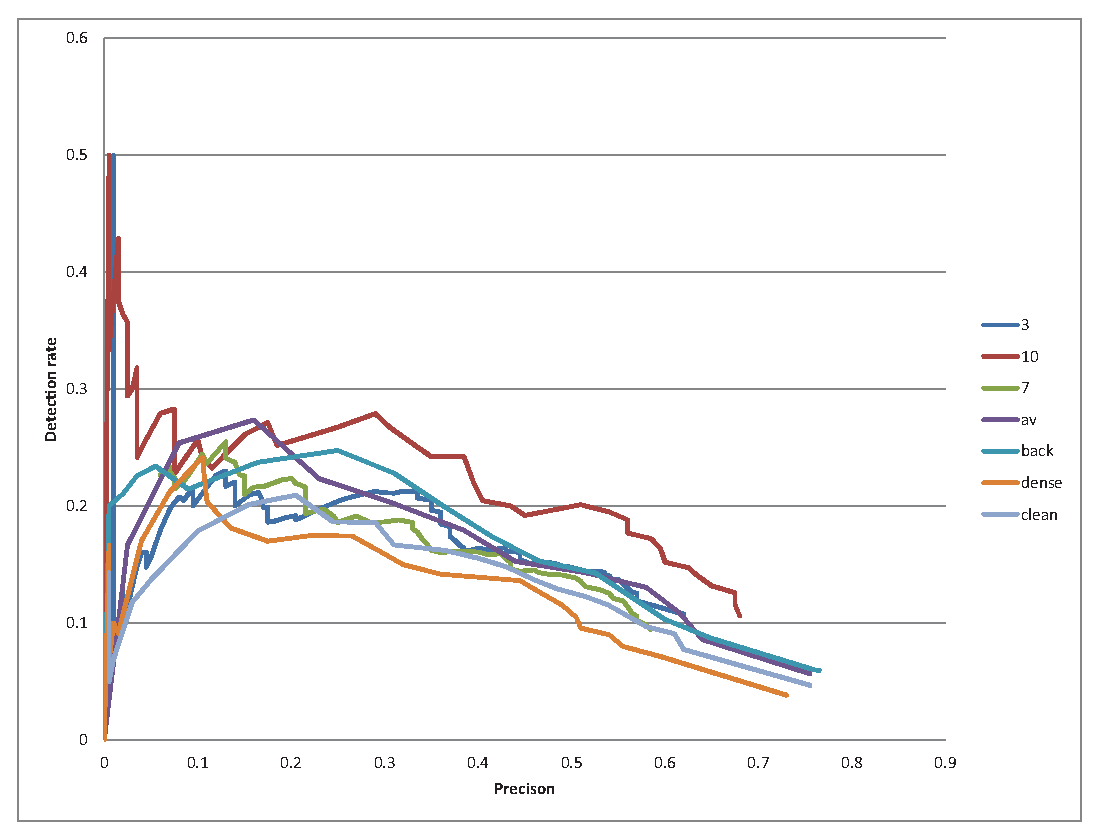
\includegraphics[width=1\textwidth]{pms.eps}


\caption[Result evaluation]{Results evaluation on UIUC cars with different implementation parameters.}
\label{fig:c52}
\end{figure}

In Figure \ref{fig:c52}, evaluations are given.

\section{Chapter Conclusion}
\label{conc5}

There will be several experiments to be summarized for this chapter, and also several experiments to be added.
